\vspace{10pt}

{\centering\subsection*{何春潘:神奇的探险之旅}}

\addcontentsline{toc}{subsection}{何春潘:神奇的探险之旅}

\renewcommand{\leftmark}{何春潘:神奇的探险之旅}

\begin{figure}[htbp]

\centering

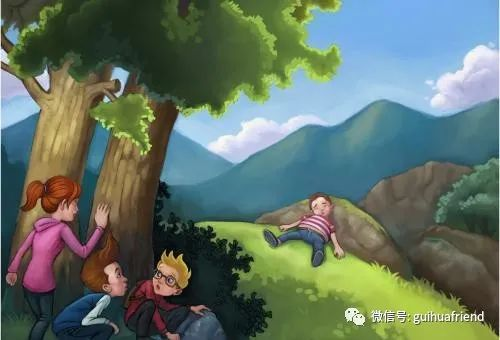
\includegraphics[width = .5\textwidth]{./ch/8.jpg}

\end{figure}



暑假我和经验丰富的探险爱好者王刚—他曾经探险过百慕大三角区域的外围,还有心细而胆小的同学林越一起去热带雨林探险。林越他检查作业时连一个笔画写错了都会圈出来,但他很胆小,怕蜘蛛。

我们带的装备有指南针、手机、充电宝、饮用水、食物、药品、帐篷、衣服、百科全书、行李箱、卫生用品、打火机、高压水枪、喷火枪、酒、风油精、防毒面具、镰刀、热熔枪、雄黄粉等等。

我们刚进入雨林,发现这里有各种各样的生物,如:老虎、多哥蜘蛛、鹿、蛇等。林越一看见蜘蛛就吓得大叫起来,把我们都吓了一跳。我们心都提到嗓子眼儿上。

我们走到雨林中外围发现了一只眼镜蛇,而我们不小心惊动了它,它便朝我们爬来,我吓得不敢出声,赶忙拿出雄黄粉泡的酒,再拿出高压水枪,把高压水枪对准眼镜蛇,把雄黄酒喷在眼镜蛇上,眼镜蛇立马被赶跑了。他们都夸我反应能力快。

可是王刚却说:“刚闹出这么大动静,以我多年的探险经验,我们要赶快走了,不然会引出其他生物过来。”

我们继续往前走,发现了一群蚂蚁在筑巢,王刚却说不是在筑巢。因为里面既有红火蚁又有白蚁,应该是红火蚁在抢夺白蚁的巢穴。林越说:“我发现了个问题,百科全书上明明说红火蚁在什么地方,一百米范围内必有一座红火蚁蚁穴,且还有一只红火蚁蚁后。”“我们先不管他们,跟着红火蚁走一定能找到红火蚁巢穴。”王刚说。我们走过去果真发现了一处蚁穴。我赶忙把高压水枪中装酒的瓶换成水瓶,直接摧毁了这座蚁穴。

几天后,我们的粮食没有了,我们已经饿了一天了,终于在我们精疲力尽时发现了一处天然香蕉树。我们赶忙跑过去,可是却发现有一只好大的多哥在树上,体型比我头还大,我直接把高压水枪里的水瓶换成酒瓶后,将喷火枪对准高压水枪喷出去的酒,这样酒就燃了,最终那只蜘蛛被烧死了。我们用镰刀割下香蕉吃了起来,然后依靠手机导航走出了雨林。

我觉得这次探险好刺激,而且全员归来,这些重重经历让我知道了遇到事情不要慌张,要冷静思考打破常规。我得到的知识实在太多了,足以让我受益一生。





\vspace{10pt}



作者:五(3)班 何春潘



指导老师:刘婷



投稿:2021年6月8日



发表:2021年6月8日










                



\vspace{10pt}

\hline



